\documentclass{report}

\usepackage[utf8]{inputenc}
\usepackage[T1]{fontenc}
\usepackage[francais]{babel}
\usepackage{hyperref}
\usepackage{verbatim}
\usepackage{titlesec, blindtext}
\usepackage{microtype}
\usepackage{graphicx}
\usepackage{xcolor}
\usepackage{listings}
\usepackage{textpos}
\usepackage{float}
\usepackage{biblatex}
\addbibresource{sample.bib}
\usepackage[left=2.5cm,right=2.5cm,top=1.5cm,bottom=1.5cm]{geometry}
\graphicspath{{images/}}
\newcommand{\hsp}{\hspace{10pt}}
\titleformat{\chapter}[hang]{\Huge}{\thechapter{.}\hsp}{0pt}{\Huge}

\lstdefinestyle{code}{keywordstyle=\color[rgb]{0.627,0.126,0.941},commentstyle=\color[rgb]{0.133,0.545,0.133},stringstyle=\color[rgb]{01,0,0},}
\lstdefinestyle{numbers} {numbers=left, stepnumber=1, numberstyle=\small, numbersep=10pt}
\lstdefinestyle{MyFrame}{frame=lines}
\lstdefinestyle{bashStyle} {language=Bash,style=numbers,style=MyFrame,style=code}
\lstdefinestyle{rubyStyle} {language=Ruby,style=numbers,style=MyFrame,style=code}

%\begin{lstlisting}[style=bashStyle]
%#include<stdio.h>
%main() {
% printf("Hello World");
%}
%\end{lstlisting}

\title{
    \begin{textblock}{\textwidth}(0,-0.5)
        \begin{flushleft}
            \includegraphics[width=250]{um}
        \end{flushleft}
    \end{textblock}
    \begin{textblock}{\textwidth}(0,-1)
        \begin{flushright}
            \includegraphics[width=90]{fds}
        \end{flushright}
    \end{textblock}
    \vspace{3 cm}
    \begin{minipage}\linewidth
    \vspace{3 cm}
        \huge\centering{
            RAPPORT DE PROJET\break
            Prise en main d'un environnement de Cloud : OpenStack
        }
        \vspace{1 cm}\bigbreak
        \includegraphics[width=175]{OS}
    \end{minipage}
}
\author{%
    \begin{minipage}\linewidth
        \centering{
            Groupe : \break
            BENAIS Charles,\break
            BRESSAND Jérémy,\break
            CULTY Alexandre,\break
            ROGLIANO Théo\bigbreak
            Tutrice : BOUZIANE Hinde
        }
    \end{minipage}
    \vspace{1 cm}
    \date{2015 - 2016}
}
\begin{document}
%\tracingall %ajoute info debug

\maketitle % Page de garde

\tableofcontents % Table des matières

\large % Pour la taille de la police


% -------- REMERCIEMENTS ----------
\newpage
\chapter*{Remerciements}
    Nous tenons tout d'abord à remercier Mme.BOUZIANE Hinde, notre tutrice de projet, qui nous a permis de réaliser ce projet dans de bonnes conditions.\bigbreak

    Nous voulons aussi remercier l'équipe Grid5000 qui nous à permis de réaliser ce projet sur leur plateforme distribuée par l'intermédiaire de notre tutrice, ce qui nous à offert la possibilité de réaliser ce projet dans un environnement réaliste et adapté à la notion de cloud computing.



% -------- INTRODUCTION ----------
% -------------	1 ----------------
\newpage
\chapter{Introduction}

    \begin{quote}
        \textit{«Le Cloud Computing est l'ensemble des disciplines, technologies et modèles commerciaux utilisés pour délivrer des capacités informatiques (logiciels, plateformes, matériels) comme un service à la demande.» \cite{cloud_computing}}
    \end{quote}
    \bigbreak

    Le Cloud est né à la suite de la multiplication des centres de données, de l'expension des communications et de la vitesse des calculs ainsi que de la maitrise de la virtualisation.

    \bigbreak

    Avec les systèmes Unix la virtualisation s'intègre à la couche matérielle et permet la communication avec le Kernel, cela consiste à offrir une certaine souplesse dans l'utilisation des ressources de son infrastructure informatique.\newline
    Le Cloud (OpenStack) vient s'intégrer à la couche de virtualisation du système et offre une interface pour la réservation de capacités de calcul et de stockage ainsi que son orchestration.\newline
    Ce point de vue offre les aspects fondamentaux de l'infrastructure en tant que service (Infrastructure as a Service ou IaaS), celle qui nous intéressera ici en particulier, et permet la mise en place d'autres services plus spécialisés, présentés succinctement dans la figure ci-dessous.

    \begin{figure}[H]
        \centering{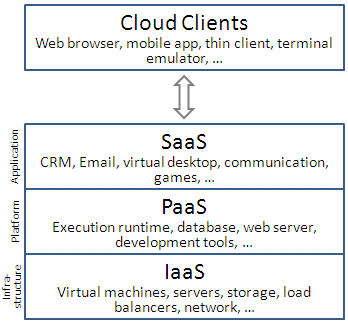
\includegraphics[scale=0.8]{Cloud_computing_layers}}
        \caption{Les différents niveaux de Clouds \cite{wiki_IaaS}}
    \end{figure}

    De grandes entreprises offrent des Web-Service similaire en proposant la location d'une partie de son infrastructure informatique (le Cloud public avec par exemple Amazon avec Elastic Compute Cloud (EC2), Microsoft avec Azure et Google).\newline
    Présentons OpenStack, la problématique et les objectifs de notre projet, ainsi que l'organisation mise en place.

    \section{L'environnement de cloud OpenStack}

        \begin{quote}
            \textit{«OpenStack est un ensemble de logiciels open source permettant de déployer des infrastructures de cloud computing (IaaS). La technologie possède une architecture modulaire composée de plusieurs projets corrélés (Nova, Swift, Glance...) qui permettent de contrôler les différentes ressources des machines virtuelles telles que la puissance de calcul, le stockage ou encore le réseau inhérents au centre de données sollicité.»
            \cite{wiki_openstack}}
        \end{quote}

        \bigbreak

        Un environnement de cloud de type IaaS permet de créer des machines virtuelles avec des ressources réservées sur lesquelles l'utilisateur pourra installer le système d'exploitation et les applications qu'il souhaite. Par exemple, OVH et Online sont des entreprises offrant ce service à travers des offres de location de serveurs virtuels (Virtual Private Server ou VPS).

        %############################################
        % ##### Faire une introduction sur l'image !!, et idem que l'autre, elle n'est pas très parlante je trouve
        \begin{figure}[H]
            \centering{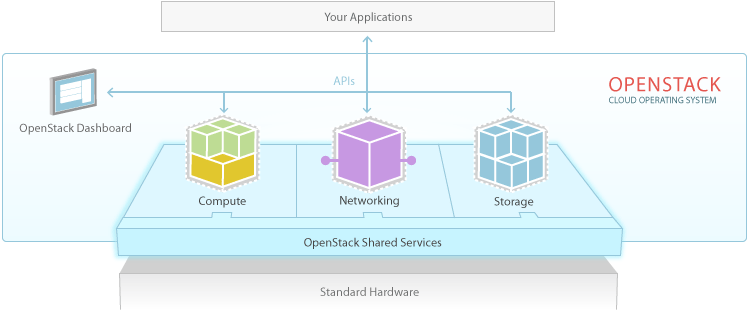
\includegraphics[width=\linewidth]{openstack-software-diagram}}
            \caption{OpenStack Software \cite{openstack_software}}
        \end{figure}


        OpenStack est à ce jour composé de 17 logiciels (modules) mais nous nous intéresserons à un seul : Nova.
        \begin{quote}
            \textit{«Nova dirige le cycle de vie des instances de calcul dans un environnement OpenStack. Les responsabilités de Nova englobent la création, l'ordonnancement et le démantèlement des machines virtuelles sur demande.» \cite{openstack_nova}}
        \end{quote}

        \bigbreak

        % ##############################################
        % On utilise que le commandes nova mais je pense qui y avait pas glance, ou neutron, on pourrait rien faire vu qu'on aurait pas d'OS, ni de réseau (enfin réseau optionnel)... non ?
        Nova gère la communication avec la plateforme de virtualisation (l'hyperviseur KVM plus spécifiquement) intégrée au noyau Linux, permettant l'instantiation de plusieurs machines virtuelles sur une même machine physique.
        Nova est suffisant pour créer un environnement de cloud. En effet il permet de créer un ensemble de machines virtuelles connectées au réseau publique de la machine hôte, d'y installer un système d'exploitation ainsi que des serveurs ssh par exemple pour pouvoir ensuite s'y connecter à distance et installer les applications qu'il souhaitent, et les exécuter.

    \section{Problématique et objectifs du projet}

        Ce projet a pour but de permettre la prise en main d'un environnement de cloud de type IaaS à travers OpenStack en mettant en oeuvre un sytème d'automatisation de déploiement d'applications sur des machines virtuelles.\bigbreak

        Suite à ces objectifs, nous avons défini les problèmatiques suivantes :\newline
        Comment utilisé OpenStack pour créer des machines virtuelles ?\newline
        Comment installer et démarrer des applications sur les machines virtuelles ?\newline
        Enfin, comment automatiser le déploiement d'applications sur des machines virtuelles ?


	\section{Organisation du projet}

    	Afin de mieux déterminer les tâches à effectuer, nous avons d'abord réalisé le diagramme de Gantt suivant :

    	\begin{figure}[H]
            \centering{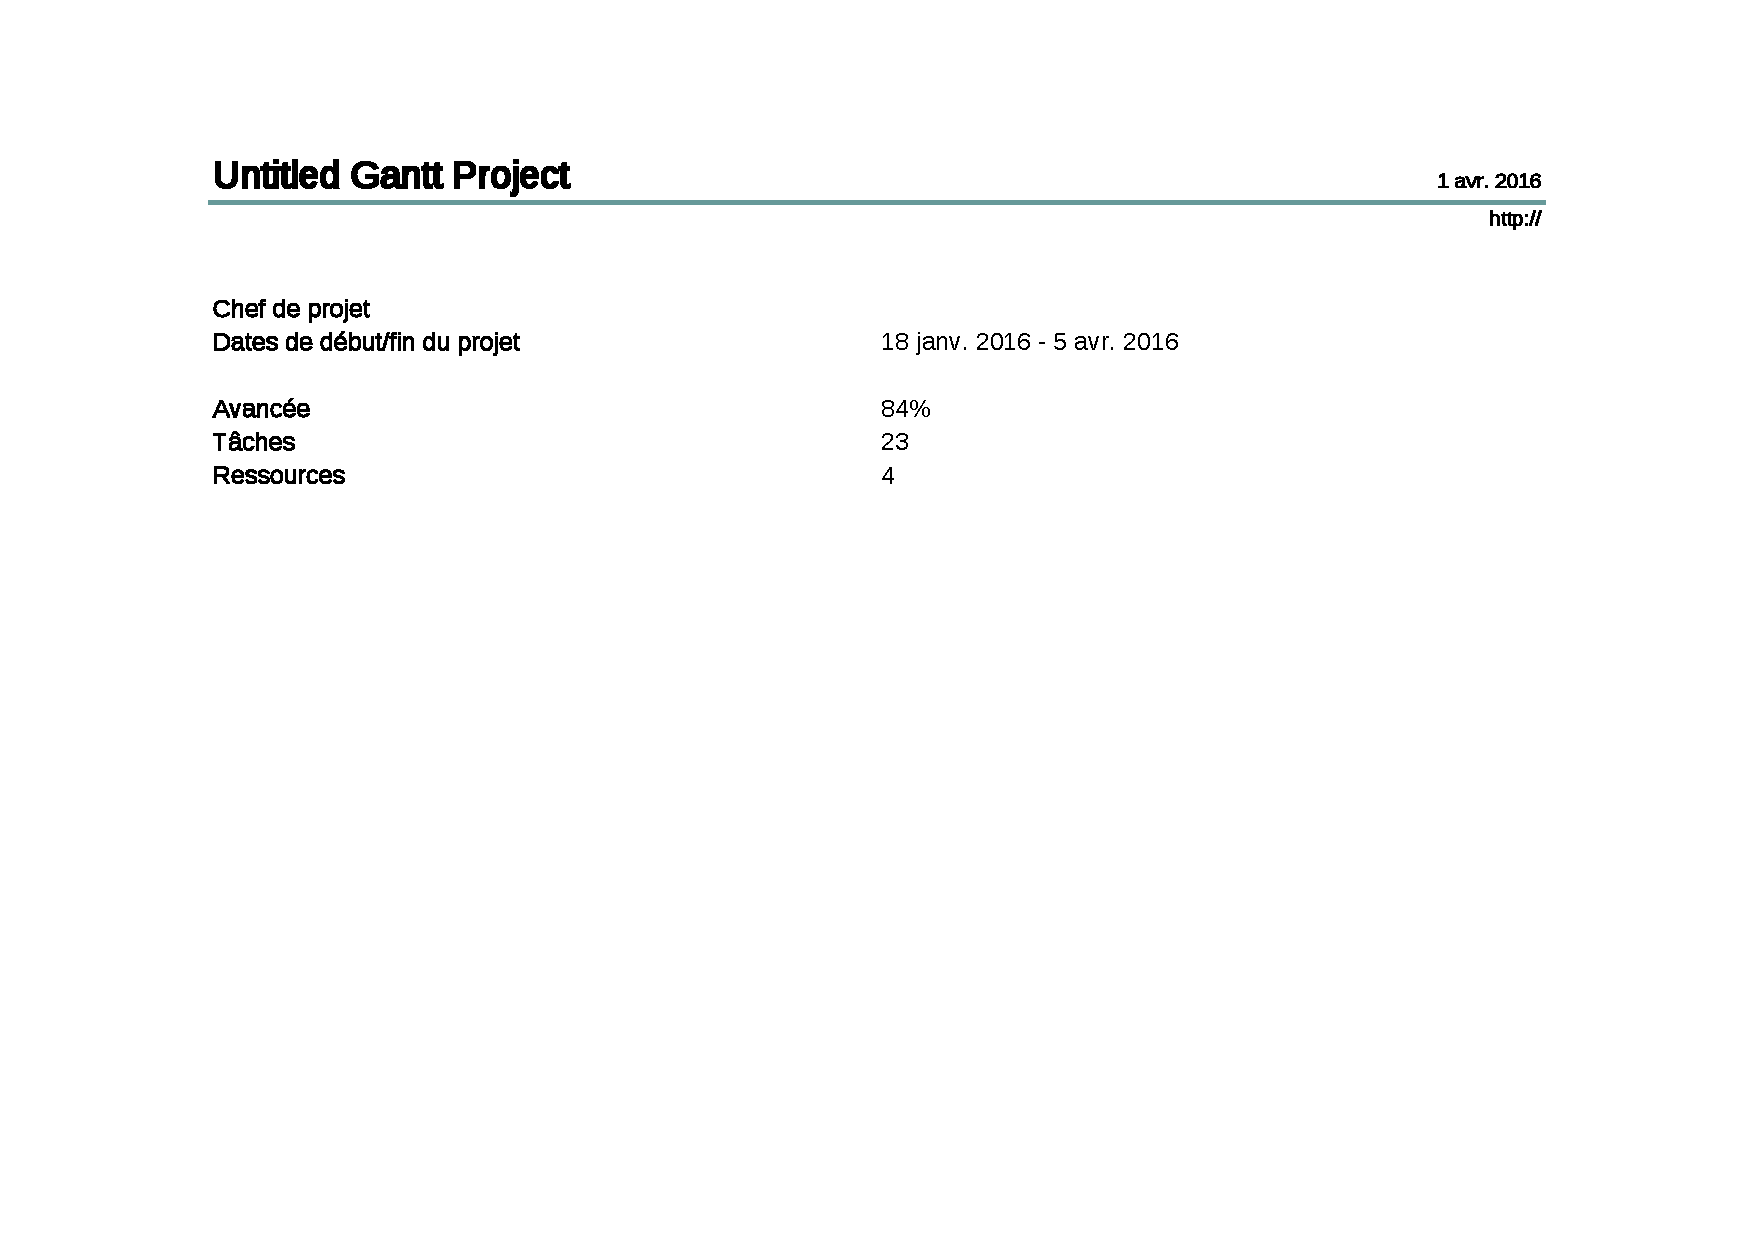
\includegraphics[width=\linewidth]{gantt}}
            \caption{Diagramme de Gantt}
        \end{figure}
    	\bigbreak

        Tout au long du projet nous nous sommes réunis en moyenne deux après-midi par semaine pour travailler.
        Nous tenions aussi une réunion hebdomadaire avec notre tutrice de projet afin de l'informer de nos avancements et de lui demander des conseils.

        \bigbreak

    	%Plan du rapport ( paragraphe ou plan numéroté ?)
        Dans la suite de ce rapport nous présenterons la prise en main de l'environnement OpenStack à travers nos premières expériences. Ensuite, nous développerons le travail effectué, et notamment la conception de l'outil permettant le déploiement d'applications sur des machines virtuelles. Enfin nous terminerons par un bilan de ce projet Cloud Computing à travers OpenStack.


% -------- CONTENU ----------
% ----------- 2 -------------
\newpage
\chapter{Prise en main d'OpenStack}
		%Paragraphe introductif : On peut controler son cloud soit grace au dashboard (expliquer ce qu'est le dashboard : clic clic pouet pouet), soit grace à l'API (qu'est-ce que l'API). L'API est la seule solution pour l'automatisation<.
       Il existe deux solutions pour mettre en place et gérer son cloud avec Openstack. La première est une interface utilisateur basée sur des pages web pour gérer les differents services (Nova, Neutron, ...) apellée dashboard (en français tableau de bord). C'est le service Horizon. La deuxième est de passer par une interface de programmation applicative (souvent désignée par le terme API pour Application Programming Interface). C'est un ensemble normalisé de classes, de méthodes ou de fonctions qui sert de façade par laquelle un logiciel offre des services à d'autres logiciels. Afin d'atteindre notre but d'automatisation, nous avons choisi d'utiliser l'API  offrant plus d'outils pour y parvenir.\bigbreak

      %Un aperçu de l'interface utlisateur se trouve disponible en annexe page \pageref{cloudHorizon} figure \ref{cloudHorizon}.


    \section{Installation d'OpenStack sur machines personnelles}

    %objectif initial : expliquer nos objectifs lors de l'installation d'OpenStack sur nos machines
    Dans le but de déployer un environnement OpenStack nous avons choisi d'utiliser DevStack, un projet qui a pour but de rendre l'installation d'OpenStack accessible (avec peu de près-requis) avec un script permettant le téléchargement et la configuration de tous les composants essentiels à OpenStack.\newline
     %ajouter dans bib lien github/devstack:
    Nos objectifs étaient de déployer OpenStack sur nos machines de manière individuelle dans un premier temps puis de déployer OpenStack sur un réseau comprenant l'ensemble de nos machines.

    \bigbreak

    Il est conseillé d'utiliser DevStack sur des machines virtuelles car DevStack modifie la configuration réseau et la configuration des droits d'accès aux fichiers sur les machines physiques hôtes.\newline
    De plus, DevStack doit être redéployé à chaque démarrage de la machine hôte, ce qui constitue une contraite supplémentaire.\newline
    Face à celles-ci, notre tutrice nous a offert la possibilité d'utiliser d'un environnement OpenStack dédié à une plateforme distribuée existante nommée Grid5000 et présentée dans la section suivante.

    \section{OpenStack sur une plateforme distribuée}

		\subsection{La plateforme Grid'5000}

La plate-forme Grid’5000 est une grille informatique, c’est-à-dire une infrastructure distribuée sur différents sites géographiques répartis principalement en France (Grenoble, Lyon, Toulouse, Bordeaux, Lille, Rennes, Reims, Nantes, Nancy, Luxembourg).
Elle a été créée par une initiative de l'INRIA.
%ajouter bib lien vers G5K

\bigbreak

 Elle dispose de 1171 nœuds physiques. La totalité des nœuds représentent 2218 processeurs, soit  8000 cœurs. Les sites géographiques sont reliés par une fibre optique 10 Gbits/s faisant partie du réseau RENATER qui relie les différentes universités et centres de recherche français.

 \bigbreak

\begin{figure}[H]
        \centering{\includegraphics[scale=0.45]{grid5000}}
        \caption{Architecture de Grid'5000}
        \label{grid5000}
        \hspace{\linewidth}
        \textbf{source : }www.grid5000.fr/mediawiki/index.php/Getting\_Started
\end{figure}

Le point d'entrée à l’infrastructure G5K est acces.grid5000.fr et se fait via SSH, permettant d’accéder aux différents sites sur lesquels il est possible d’effectuer des réservations de noeuds.
\bigbreak

		  \subsection{OpenStack sur Grid'5000 : XP5K-OpenStack}

		     \begin{quote}  %%%%%%% à reprendre
                «XP5K est une bibliothèque légère écrite en Ruby permettant d'aider les utilisateurs de Grid'5000 à préparer leur expérimentations en faisant appel à l'interface de programmation Grid'5000 pour :
                \begin{itemize}
                \item Faire des réservations, voir le statut des réservations, supprimer une réservation...
                \item Créer des rôles (chaque nœud est dédié à un rôle, par exemple : contrôleur, unités de calcul), sans avoir à connaître le nom des nœuds qu'on utilise.
                \item Faire un ou plusieurs déploiement sur des nœuds spécifiés par une réservation ou un rôle.» \cite{XP5K}
                \end{itemize}
            \end{quote}

            \begin{quote}
		       «Puppet est un logiciel libre, écrit en Ruby, permettant la gestion de la configuration de serveurs esclaves. Il permet de gérer les déploiements système et applicatif.»
		       \cite{Puppet}
		    \end{quote}

            XP5K-OpenStack est une interface de programmation conçue pour déployer OpenStack sur Grid'5000.
            XP5K-OpenStack utilise d'une part l'interface de programmation XP5K, permettant de manipuler les réservations et les nœuds sur Grid'5000, d'autre part l'outil de gestion de configuration Puppet configuré avec les modules Puppet d'OpenStack qui, à partir d'un nœud maitre (puppet master) permet le déploiement d'OpenStack sur un ensemble de nœuds de calcul (esclave).

		  \subsection{Déploiement et exécution d'applications sur XP5K-OpenStack}
Après avoir compris les bases et le fonctionnement sur XP5K-OpenStack, nous avons commencé à réfléchir aux moyens d'installer et d'éxécuter une application sur un cloud. Celà permettra de lister les étapes nécessaires et identifier lesquelles nous pourront automatiser par la suite.\bigbreak

Une fois connecté sur Grid'5000 et XP5K-OpenStack importé sur le compte utilisateur, il faut l'éxécuter afin que celui ci déploie Openstack sur les noeuds réservés (durée de cette étape ~30 minutes).\bigbreak

À partir de maintenant, nous avons tous les outils pour créer/gérer le cloud. Il nous faut créer et paramétrer les machines virtuelles sur lesquels nous allons déployer nos applications. Cela fait, il ne nous manque plus qu'à importer les fichiers nécessaires à l'installation ou directement l'éxécutable sur les machines virtuelles précédemment créées. Il est à noter que nous utiliseront des images Unix sur nos machines virtuels, les applications doivent donc être portable ou du moins compatible.
La dernière étape étant simplement d'installer et d'éxécuter la ou les applications.

		  %se connecter au site

		  %cloner xp5k-OpenStack

		  %creer les VM

		  %copier les fichiers sur la VM

		  %executer les programmes sur les VM


    \section{Réfléxion sur l'automatisation}
    Bien qu'il soit techniquement possible de tout automatiser, certaines parties sont plus avantageuses que d'autres. Tout ce qui est lié à Grid'5000 étant plus spécifique à notre situation, l'automatisation de cette partie semble moins intéressante et moins au coeur du projet.
    Par contre, rendre le paramétrage et la création des machines virtuelles ainsi que l'installation et l'éxécution d'application automatique est l'essentiel de notre projet. Nous nous sommes donc concentrés à réaliser cette tâche.

		%(falcutatif)



% -------- CONTENU ----------
% ----------- 3 -------------
\chapter{Un outil pour automatiser le déploiement et l'exécution d'applications sur OpenStack}

Afin de réaliser cette tâche, nous avons décidé de créer des "scripts" écrits en Bash et en Ruby. Un script est un code interprété qui à la manière d'un script au théatre édicte une sucession d'actions à réaliser. Les scripts nous servent à exécuter et coordonner les comamndes de Nova automatiquement.

	%Paragraphe introductif : Quels sont les solutions techniques pour automatiser les tâches citées précedement afin de cacher les aspect techniques à l'utilisateur?

    Dans un premier temps nous verrons l'aspect algorithmique puis ensuite l'aspect technique des scripts développés.


    \section{Description générale}

    %algo : parser le fichier de configuration en un tableau
    %parcourir le tableau et creer les VM et installer les applications sur les VM
    La première étape du processus d'automatisation est la création d'un fichier de configuration structuré, contenant les informations sur les machines virtuelles ainsi que sur les applications devant y être installés.\bigbreak

    Une fois que ce fichier de configuration est créé, alors on démarre le script qui analyse ce fichier et organise les informations en tableau. Ce tableau est constitué de plusieurs niveaux, le premier représentant les machines virtuelles et le second niveau représentant les applications liées à une machine virtuelle.\bigbreak

    Le script parcourt ensuite le tableau et pour chaque machine virtuelle il commence par appeler le script de création d'une machine virtuelle, puis pour chaque application il appelle le script d'installation et d'exécution d'une application.\bigbreak

    Vous trouverez en annexe page \pageref{construct}, figure \ref{construct} l'algorithme du script principal, page \pageref{vmsetup}, figure \ref{vmsetup} l'algorithme du script de création d'une machine virtuelle, et page \pageref{appsetup}, figure \ref{appsetup} l'algorithme d'installation et d'exécution d'une application sur un machine virtuelle. \bigbreak

    %algo installation d'application : transferer les fichiers sur la VM
    %se connecter a la VM
    %lancer le programme d'installation


    \section{Technologies utilisées}

    %JSON, RUBY, BASH, SCP/SSH
    Pour réaliser notre projet nous avons dû prendre en main différents outils de base :
    \begin{itemize}
        \item SSH : pour naviguer de notre machine personnelle vers les machines du réseau Grid'5000 et entre les différentes machines virtuelles.
        \begin{quote}
            «SSH signifie Secure SHell. C'est un protocole qui permet de faire des connexions sécurisées (i.e. chiffrées) entre un serveur et un client SSH.»
            [http://formation-debian.via.ecp.fr/ssh.html]
        \end{quote}
        \item SCP : pour transférer nos fichiers de notre machine personnelle à notre réportoire sur un site géographique du réseau Grid'5000, et par la suite transférer ces fichiers sur nos machines virtuelles.
        \begin{quote}
            «Secure copy (SCP) désigne un transfert sécurisé de fichiers entre deux ordinateurs utilisant le protocole de communication SSH»
            [https://fr.wikipedia.org/wiki/Secure\_copy]
        \end{quote}
        \item JSON : pour permettre à l'utilisateur de spécifier l'architecture qu'il souhaite mettre en place avec la configuration des applications et des machines virtuelles, le tout dans une syntaxe simple d'utilisation, et pouvoir récupérer ces informations dans des variables de manière structurée sous forme de tableau et de dictionnaires de données.
        \begin{quote}
            «JSON (JavaScript Object Notation – Notation Objet issue de JavaScript) est un format léger d'échange de données. Il est facile à lire ou à écrire pour des humains. Il est aisément analysable ou générable par des machines.»
            [http://www.json.org/json-fr.html]
        \end{quote}
    \end{itemize}


    \section{Implémentation}

    %Expliquer le JSON

    %montrer le parcours du tableau en ruby

    %montrer creation VM et installation app en bash
VM\_launcher est le premier script que nous avons développé. Il a pour but d'automatiser la création d'une VM, lui associer une adresse IP publique et ouvrir une plage de port pour la communication réseau. Pour cela, nous avons créé un script écrit en Bash exécutant la commande "nova boot" pour créé une machine virtuelle, la commande "nova floating-ip-create/add" créant et associant une IP à la machine nouvellement créé, et enfin la commande "nova secgroup-rule-add" pour ouvrir des ports.\bigbreak

APP\_installer vient dans la continuité de VM\_launcher. Après avoir créer une VM nous souhaitons en effet y déployer au moins un programme. C'est le rôle d'APP\_installer il installe et démarre un programme. Afin d'y parvenir, nous récupérons les adresses des VM via le controller, puis pour chaque IP récupéré nous copions les fichiers nécessaires à l'installation grâce à la commande SCP, puis installons et démarrons le programme comme si nous étions dans un terminal.\bigbreak

Enfin pour permettre le déploiement automatique, nous avons créé le script 'construc' en ruby. C'est le script qui parcourt le fichier de configuration JSON, et appelle VMSetup et appSetup, les scripts légérement modifié de VM\_launcher et APP\_installer qui ont été adapté pour le déploiement automatique.\bigbreak

    \section{Expérimentation}

    %Comment vérifier que les VM ont bien été crées et que les adresses ip ont bien été créées et attribuées.
Lors de l'éxécution de nos scripts, il est nécessaire de vérifier si chaque étape s'est déroulée correctement. Les plus importantes étant, dans un premier temps, la création des machines virtuelles et celle des adresses IP ainsi que l'association de ces dernières aux machines, et dans un second temps, l'installation et l'éxécution des programmes.\bigbreak

Pour les premières étapes à vérifier, Nova nous fournit deux commandes. La première: nova floating-ip-list, permet de voir la liste des IP créées. La seconde: nova list, permet de voir les machines virtuelles créées ainsi que leurs caractéristiques, notamment si une IP a été liée à une machine.\bigbreak

%peut être rajouter ce que les 2 comamndes affichent en image

Pour les autres étapes, nous supposons que les programmes s'installent bien ou qu'ils aient eux-mêmes prévu ce qu'ils doivent faire en cas d'échec (désintallation, nouvelle essai, etc...). Il est tout de même possible de vérifier qu'un programme est présent sur une VM en se connectant à celle-ci et en regardant par soi-même.\bigbreak

%Comment vérifier que les programmes ont bien été exécutés.
Pour vérifier l'éxécution d'un programme, il y a principalement  deux façons de faire, la plus simple étant de récupérer un résultat retourné ou un fichier de log. L'autre façon étant de se connecter à la machine virtuelle et de vérifier les processus actifs (par exemple: ps -ef | grep le nomDuProg).\bigbreak


    \section{Améliorations}

    %screen
    Pour naviguer d'une machine virtuelle à l'autre, l'utilisateur doit savoir utiliser les commandes SSH.
    Au lieu de cela, on pourrait faciliter la navigation entre les machines virtuelles en utilisant le programme Screen.
    \begin{quote}
        «Screen (GNU Screen) est un « multiplexeur de terminaux » permettant d'ouvrir plusieurs terminaux dans une même console, de passer de l'un à l'autre et de les récupérer plus tard.»
        [https://doc.ubuntu-fr.org/screen]
    \end{quote}
    Screen permet d'afficher plusieurs terminaux virtuels sur une même fenêtre, comme on peut le voir sur l'image en annexe page \pageref{screen} figure \ref{screen}.
    L'idée serait d'utiliser cette fonctionnalité pour afficher sur le même écran différents terminaux virtuels correspondant chacun a une machine virtuelle sur laquelle s'exécute l'application.
    Screen permet l'association de plusieurs terminaux virtuels dans des sessions, et la possibilité de détacher ou de rattacher une session.
    L'idée serait d'utiliser cette fonctionnalité pour permettre à l'utilisateur de naviguer entre les applications. En étant attaché a qu'une seule session l'utilisateur n'a accès qu'aux machines virtuelles sur lesquelles s'exécute l'application et en passant  sur une autre session il n'aura accès qu'aux machibes virtuelles de cette application.
    Enfin Screen est configurable avec des raccourcis pour exécuter toutes les tâches spécifiés précédemment. On peut donc facilement créer un ensemble de raccourcis pour faciliter l'utilisation de notre programme.\bigbreak


    %puppet
    Pour configurer le déploiement de ses applications avec notre programme, l'utilisateur doit manipuler un fichier de configuration au format JSON.
    L'architecture de notre fichier de configuration JSON ne permet par l'installation d'applications complexes qui prendraient par exemple plusieurs paramètres ou qui auraient par exemple un ensemble de machines virtuelles qui communiqueraient entre elles de manière plus complexe que le cas d'une application client serveur.
    Nous pourrions améliorer l'architecture de notre fichier JSON pour prendre en compte ces difficultés cependant notre fichier JSON deviendrait plus complexe et moins facile à utiliser.
    Une solution pour configurer de manière plus simple le déploiement d'application serait d'utiliser le logiciel Puppet.
    \begin{quote}
        « C'est un outil permettant de définir et de mettre en œuvre des configurations.
        ...
       Il faut installer et configurer sur chaque machine que l'on veut « puppetiser » un client, qui se réfèrera au puppetmaster, machine sur laquelle seront stockés les manifests, qui contiennent les spécifications »
        [http://connect.ed-diamond.com/GNU-Linux-Magazine/GLMF-112/Les-sysadmins-jouent-a-la-poupee]
    \end{quote}
    Puppet permet de configurer et de déployer des applications complexes sur des machines virtuelles en les 'puppetisant', les fichiers de configuration seront présents sur un seul noeud appelé le puppetmaster.
    Puppet permet la réutilisation de configurations grâce à un système de classe que l'on peut affecter aux machines. La machine bénificiera alors de la configuration de la classe. De plus il gère la diversité des configurations grâce à des templates s'adaptant à la configuration de la machine.
    Mais Puppet reste difficile d'utilisation pour un utilisateur.
    Cependant Puppet offre la possibilité de déplacer
    les informations conçernant la configuration des machines dans une base de donnée.
    L'idée serait donc de créer une application graphique facile d'utilisation pour l'utilisateur et qui modifiera une base de données dans laquelle Puppet ira chercher les informations pour configurer les noeuds.

    %montrer comment on aurait pu faire un parseur avec Heat

    %interface graphique ( automatiser la connection au point d'accès )

    %montrer comment on pourrait faire le déploiement des applications sur nos VM avec Puppet
    % jéjé : c'est moi le puppetmaster !

% ------- Conclusion --------
% ----------- 4 -------------
\newpage
\chapter{Conclusion}
    %Résumé, aboutissements et ce qui est en cours
    Après quelques difficultés liés à l'utilisation de DevStack, nous avons réussi à nous intégrer à l'environnement de Grid'5000. Petit à petit, nous avons réalisé des scripts réalisant des parties de notre objectif, pour arriver à la fin à un script global qui permet d'automatiser le déploiement de une ou plusieurs applications sur une ou plusieurs machines virtuelles.\bigbreak

    %Faire un bilan : les difficultés et comment ça nous a permi de comprendre des trucs.

    %Finir sur une note positive : ce qu'on a retenu.
    L'utilisation de Grid'5000 nous a permis d'acquérir d'importantes notions sur les infrastructures informatiques à grandes échelles.\bigbreak

    Ce projet nous a aussi permis d'acquérir d'importantes compétences et notions dans le domaine du cloud computing et d'OpenStack dans un contexte où le cloud computing semble être omniprésent.\bigbreak


% --- RESSOURCES DOCUMENTAIRES ---
% ----------- 5 -------------
\newpage
\chapter*{Ressources documentaires}
\href{https://en.wikipedia.org/wiki/Cloud_computing}{Wikipédia} :
\url{https://en.wikipedia.org/wiki/Cloud_computing}
\bigbreak
\href{http://docs.openstack.org/developer/devstack/}{Devstack} :
\url{http://docs.openstack.org/developer/devstack/}
\bigbreak
\href{http://www.openstack.org/}{Openstack} :
\url{http://www.openstack.org/}
\bigbreak
\href{https://github.com/openstack/nova}{Nova} :
\url{https://github.com/openstack/nova}
\bigbreak
\href{https://www.grid5000.fr/}{Grid5000} :
\url{https://www.grid5000.fr/}
\bigbreak
\href{https://github.com/pmorillon/xp5k-openstack}{xp5k-openstack}
\url{https://github.com/pmorillon/xp5k-openstack}
\bigbreak
\href{http://connect.ed-diamond.com/GNU-Linux-Magazine/GLMF-112/Les-sysadmins-jouent-a-la-poupee}{Puppet}
\url{http://connect.ed-diamond.com/GNU-Linux-Magazine/GLMF-112/Les-sysadmins-jouent-a-la-poupee}


\printbibliography


% ------------------------------ ANNEXES ------------------------------
\newpage
\chapter*{Annexes}

%workpackage.
    \begin{figure}[!ht]
        \centering{}\includegraphics[width=\textwidth]{workpack}
        \caption{Liste des tâches de notre diagramme de gantt}
        \label{gantt}
    \end{figure}

%L'architecture de Grid'5000
    \begin{figure}{!ht}
        \centering{}\includegraphics[width=\textwidth]{grid5000}
        \caption{Architecture de Grid'5000}
        \label{grid5000}
        \hspace{\linewidth}
        \textbf{source : }www.grid5000.fr/mediawiki/index.php/Getting\_Started
    \end{figure}

    %algorithme création machine virtuelle
    \begin{figure}[!ht]
        \centering{}\includegraphics[width=\textwidth]{algoVMSetup}
        \caption{Algorithme de création d'une machine virtuelle}
        \label{vmsetup}
    \end{figure}

    %algorithme installation application sur VM
    \begin{figure}[!ht]
        \centering{}\includegraphics[width=\textwidth]{algoAppSetup}
        \caption{Algorithme d'installation d'une application sur une machine virtuelle}
        \label{appsetup}
    \end{figure}

     %algorithme construct
    \begin{figure}[!ht]
        \centering{}\includegraphics[width=\textwidth]{algoConstruct}
        \caption{Algorithme création de machines virtuelles, intallation et exécution d'applications sur ces machines virtuelles}
        \label{construct}
    \end{figure}

    \begin{figure}[!ht]
        \centering{}\includegraphics[width=\textwidth]{screen}
        \caption{Affichage de plusieurs terminaux virtuels sur une même fenêtre avec Screen}
        \label{screen}
        \hspace{\linewidth}
        \textbf{source : }www.noobslab.com/2014/08/split-ubuntugnome-terminal-screen-and.html
    \end{figure}

    \begin{figure}[!ht]
        \centering{}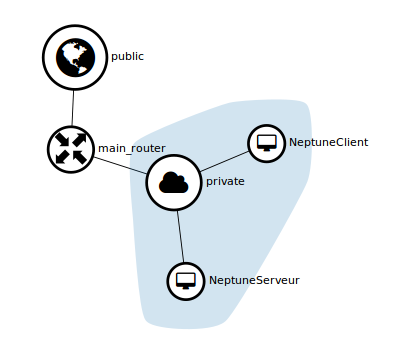
\includegraphics[width=\textwidth]{network-topo.png}
        \caption{Vue du cloud offerte par Horizon}
        \label{cloudHorizon}
    \end{figure}
\end{document}


% --------------------------- INSTALLATION LATEX ----------------------
%sudo apt-get install texlive
%sudo apt-get install texlive-lang-french
%sudo apt-get install texlive-latex-extra
% Compile Time : pdflatex Rapport.tex
% Pensez à virer les .log, .aux, .out ET .pdf avant de push !
